Rosesland cuenta con dispositivos tipo \gls{tablet}, por lo que el diseño de la interfaz de usuario debe aprovechar las ventajas que ofrece este entorno interactivo. Se pretende resumir el proceso de venta, elaboración y entrega de productos en dos secciones. También se agrega una sección de administración de usuarios y una página con información general de la florería.
\vspace{0.8cm}

La interfaz de usuario juega un papel muy importante en el aumento de la usabilidad de una aplicación, dado que la IU ofrece al usuario una vista abstracta de todo el sistema, el éxito del sistema depende en gran medida de ello. Por lo tanto, el diseño de la interfaz de usuario debe tener la importancia adecuada en el proceso del ciclo de vida del diseño del sistema.
\vspace{0.8cm}

% \begin{figure}[H]
%   \centering
%   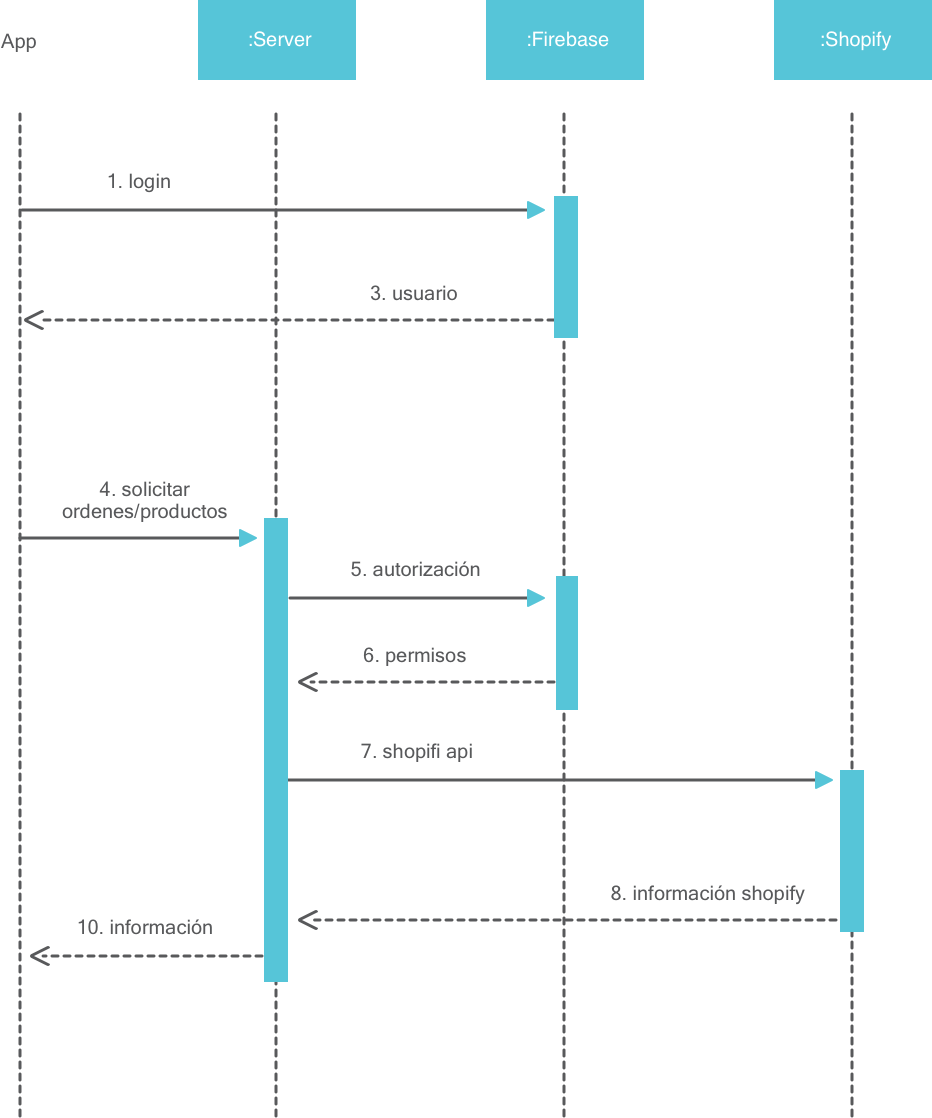
\includegraphics[width=0.75\textwidth]{secuence}
%   \caption{Diagrama de secuencia del proceso de autorización.}
% \end{figure}
% \vspace{0.8cm}
\subsubsection{Módulo de inicio de sesión}
Uno de los desafíos es cómo implementar un esquema de autenticación y autorización flexible, seguro y eficiente. Parece confuso diferenciar entre autenticación y autorización. De hecho, es muy simple.

\begin{itemize}
  \item Autenticación: se refiere a verificar `quién es usted', por lo que debe usar el nombre de usuario y la contraseña para la autenticación.

  \item Autorización: se refiere a lo que `puede hacer', por ejemplo, acceder, editar o eliminar datos a algunos documentos, esto sucede después de la verificación.
\end{itemize}

Firebase Authentication proporciona servicios de back-end, SDK fáciles de usar y bibliotecas de interfaz de usuario para autenticar a los usuarios en la aplicación. En el código ejemplo \ref{login} se muestran los métodos necesarios para el manejo de sesiones del proyecto.
\vspace{0.8cm}

\lstinputlisting[style=ES6, label=login, caption=Fragmento de código del manejo de sesión de usuario]{code/login.js}

Gracias a la simplicidad y efectividad de los servicios de Firebase, este proceso es utilizado por muchas aplicaciones y servicios web en la actualidad.
\vspace{0.8cm}

\begin{figure}[H]
  \centering
  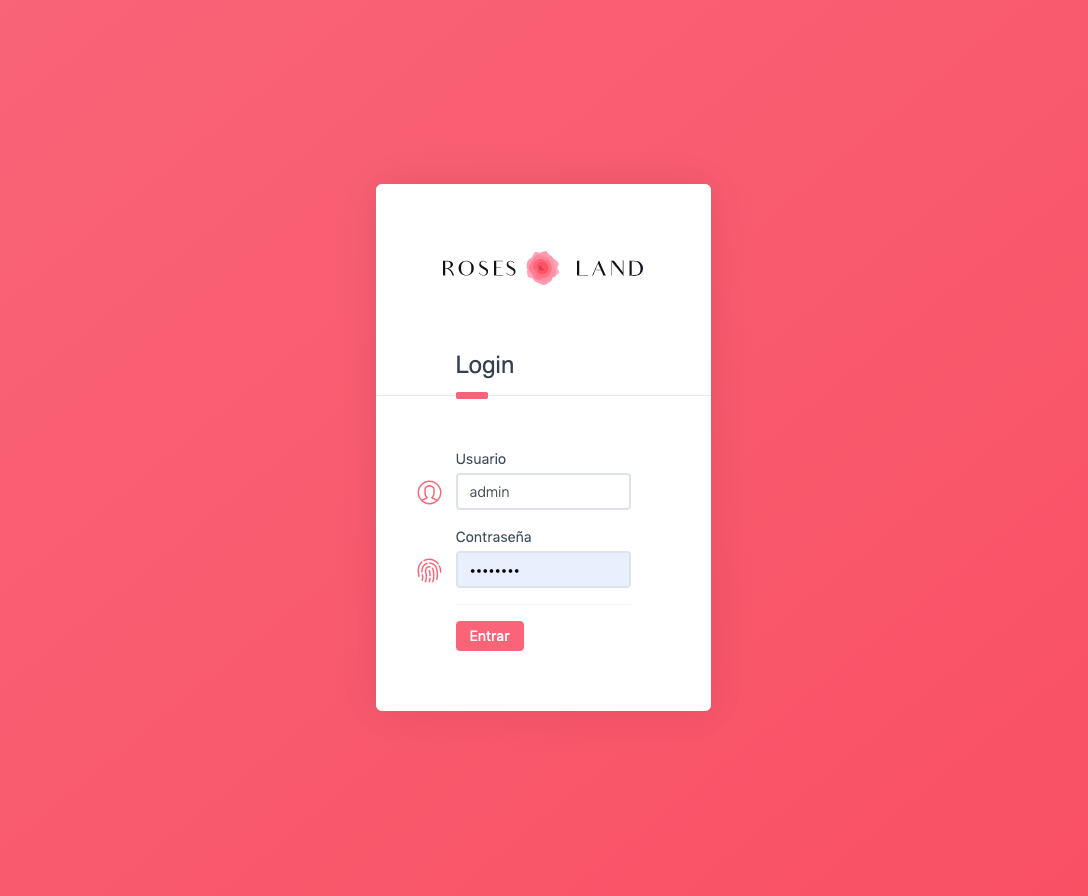
\includegraphics[width=1\textwidth]{app-login}
  \caption{Diseño final de la sección de inicio de sesión.}
\end{figure}

\subsubsection{Interfaz de usuario principal}
Después del inicio de sesión exitoso, el usuario es dirigido a la página principal que proporciona enlaces a los módulos del sistema. Esta sección contiene los componentes visuales de cada paso en el proceso de venta, manufactura y entrega, aquí se muestran todas las ordenes del día creadas mediante la conexión con Shopify, así como las creadas por la aplicación.

Este módulo permite a los vendedores asignar los floristas que elaboraran los pedidos y al administrador de logística definir los chóferes que repartirán la entrega. Las ordenes mostradas se filtran para mostrar solo la información necesaria a cada usuario en específico.
\vspace{0.8cm}

\begin{figure}[H]
  \centering
  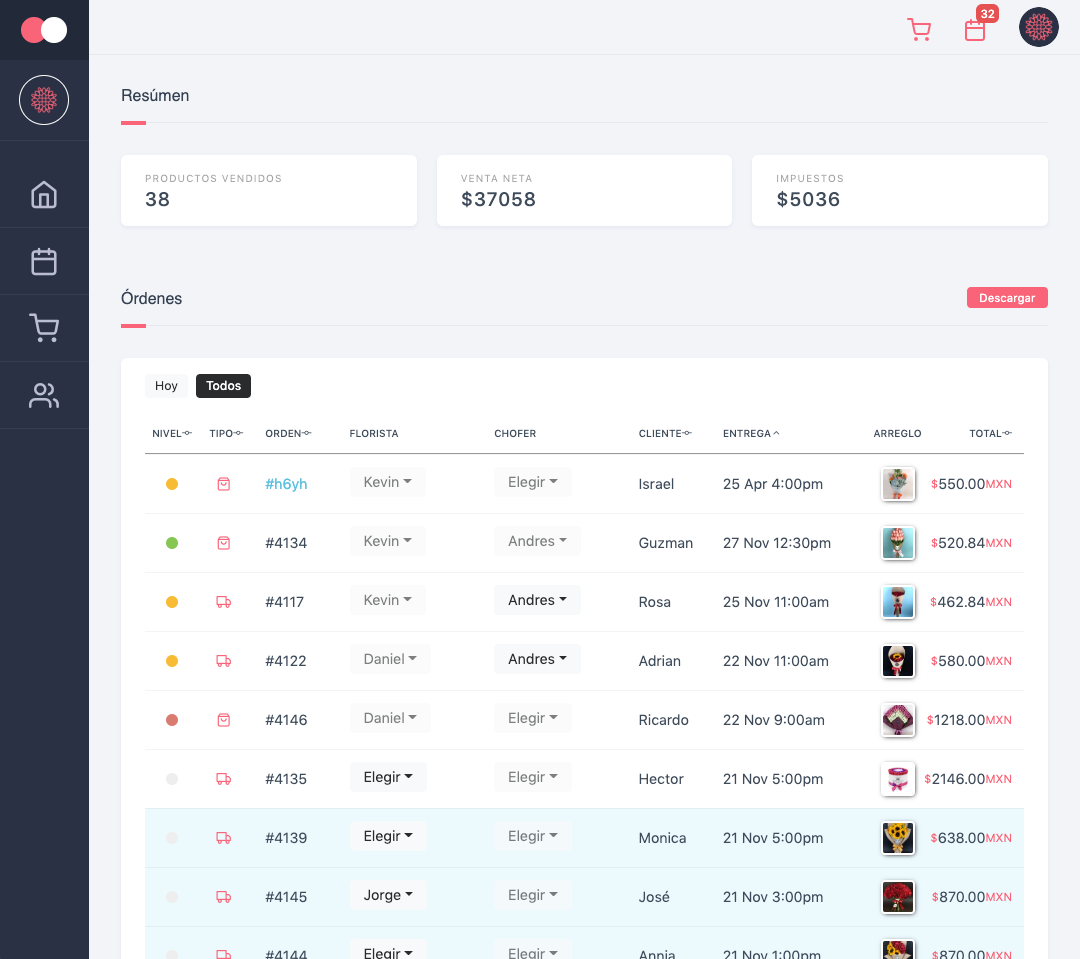
\includegraphics[width=1\textwidth]{app-main}
  \caption{Diseño final de la sección principal.}
  \label{main-ui}
\end{figure}

En la figura \ref{main-ui} se muestran los componentes principales de la interfaz de usuario (vista por el administrador). Por el lado izquierdo y en la parte superior se tienen accesos a los módulos del sistema y al perfil del usuario, El cuerpo contiene un resumen de las ventas (que solo es visible por el administrador), una tabla con la información de las ordenes del día y la opción de ver ordenes creadas para días posteriores. Las ordenes sin revisar se marcan en un tono azul y el estado de cada orden se identifica con un color:

\begin{itemize}
  \item Gris: orden pendiente.
  \item Rojo: orden iniciada.
  \item Amarillo: orden en proceso de entrega.
  \item Verde: orden finalizada.
\end{itemize}

El diseño responsivo permite al administrador llevar control del estatus de las ordenes en todas las etapas del proceso desde un dispositivo celular.
\vspace{0.8cm}

\begin{figure}[H]
  \centering
  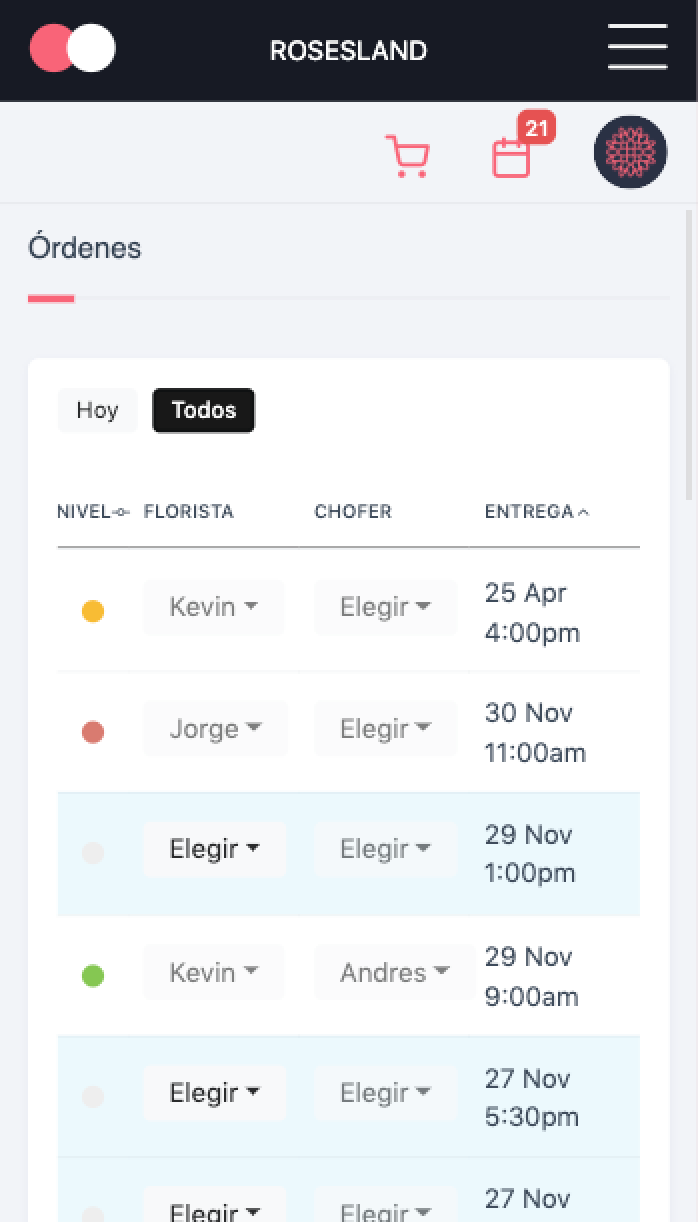
\includegraphics[width=0.4\textwidth]{app-mobile}
  \caption{Diseño de la aplicación móvil.}
\end{figure}
\vspace{0.8cm}

\subsubsection{Interfaz de usuario de la sección de ventas}
Para crear ordenes dentro del establecimiento se accede a esta sección. Aquí se seleccionan los productos, la dirección de entrega, la dedicatoria y la información del emisor y remitente de la orden. Si se llega a cometer un error con la orden una vez creada, este mismo módulo permite editarla.
\vspace{0.8cm}

\begin{figure}[H]
  \centering
  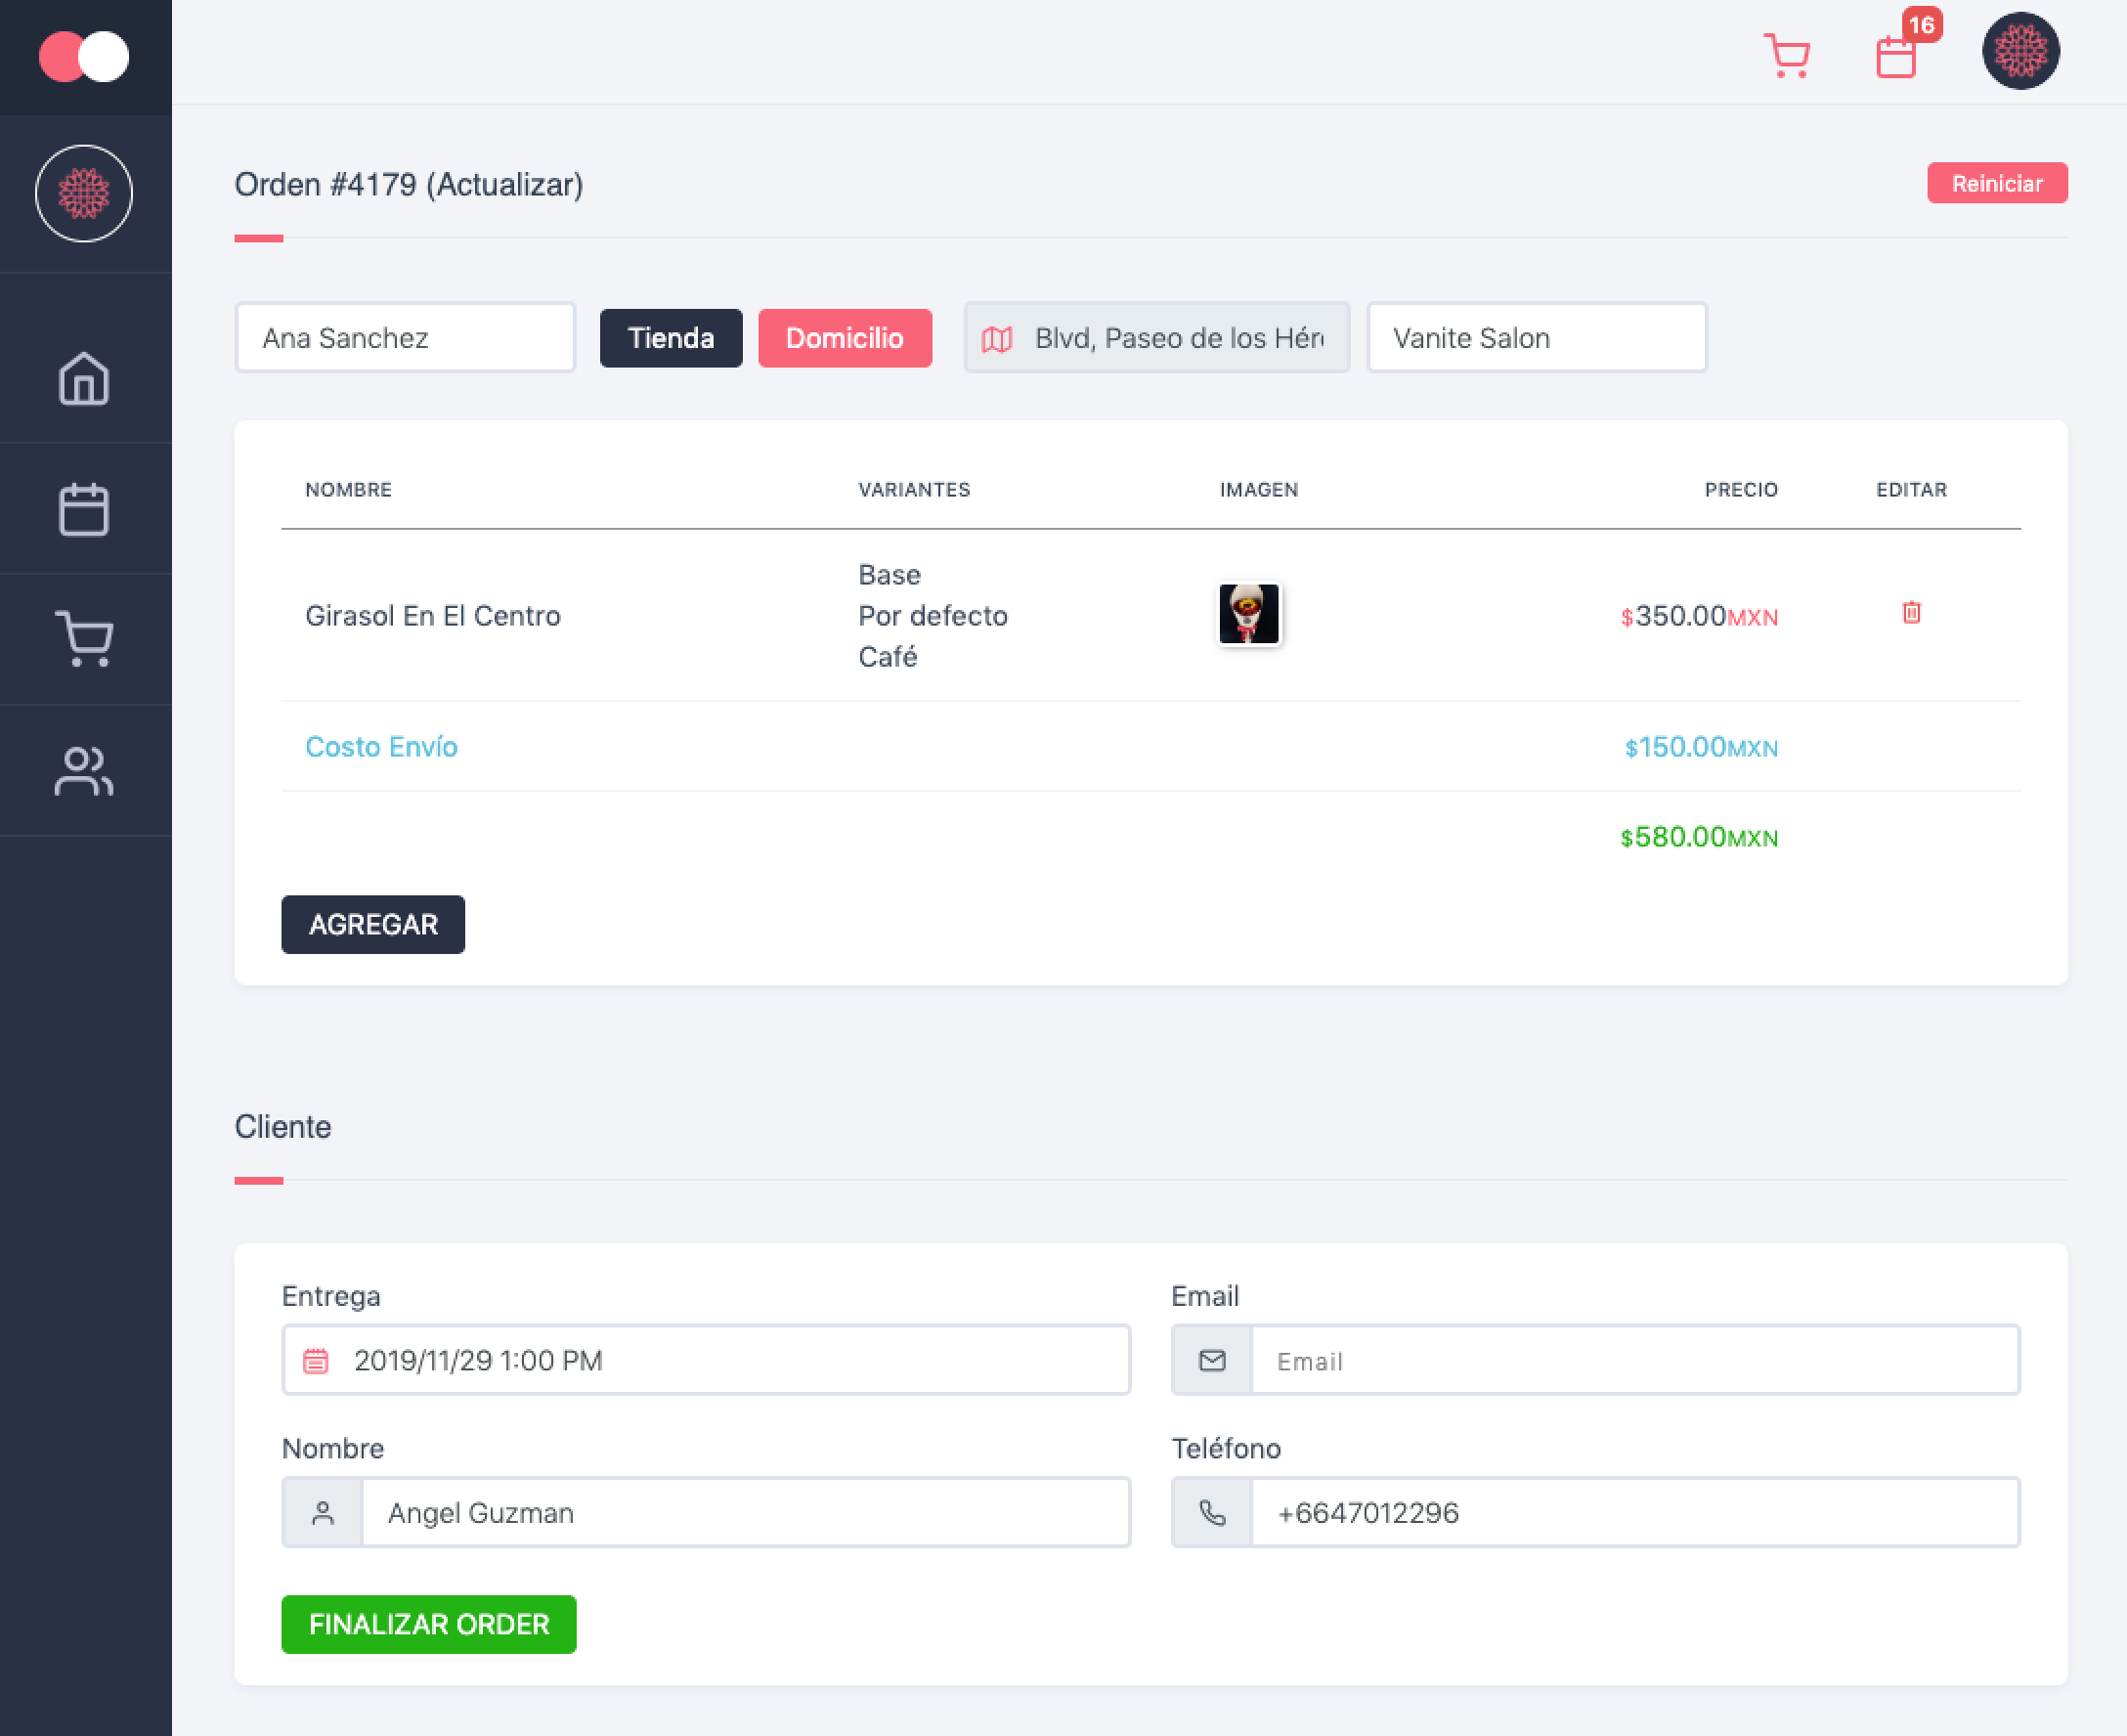
\includegraphics[width=1\textwidth]{app-sales}
  \caption{Diseño final de la sección de ventas.}
\end{figure}

El componente de catalogo de productos (figura \ref{catalog} y \ref{single-product}) se muestra en una ventana emergente que puede ser deslizada horizontalmente con el tacto, con la ayuda del mouse o haciendo clic en sus elementos. Un producto puede tener variantes de color de flor, color de papel, cantidad de flores, etc. Cada producto puede también contener extras y una dedicatoria (figura \ref{single-product}).

\begin{figure}[H]
  \centering
  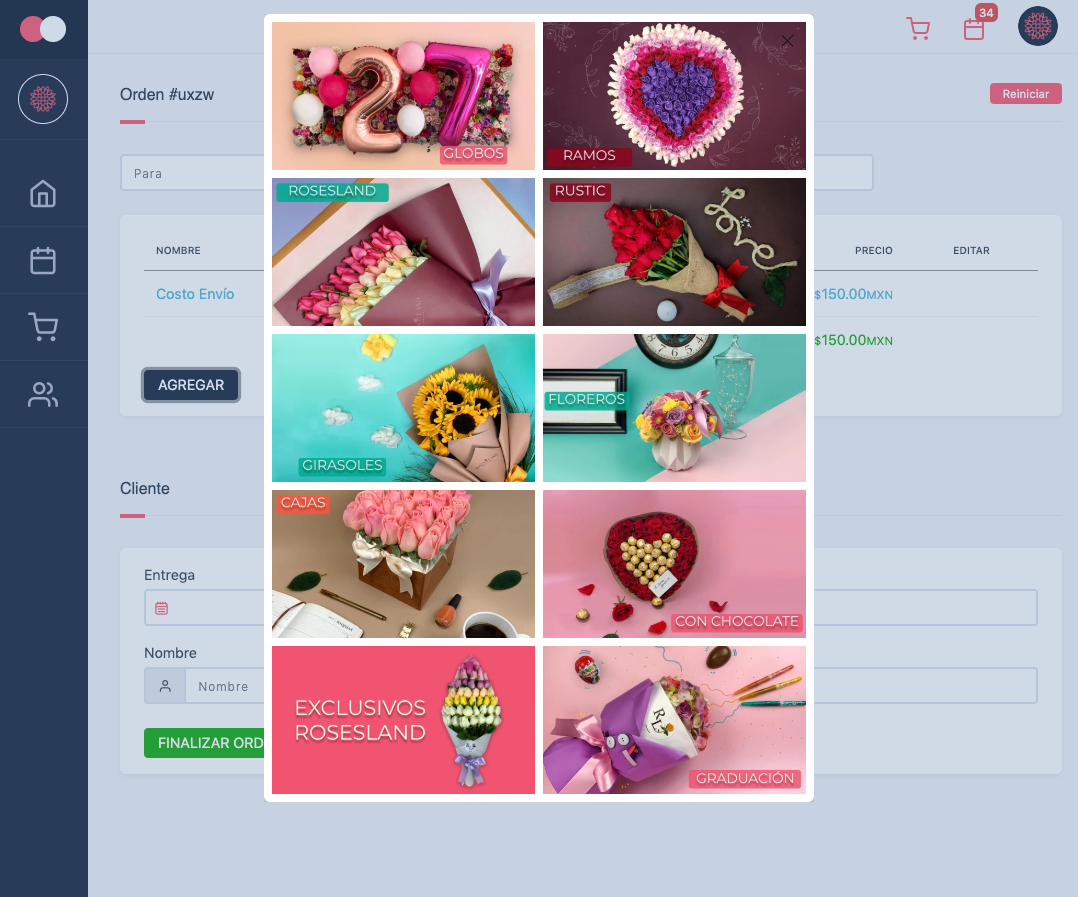
\includegraphics[width=0.6\textwidth]{app-catalog}
  \caption{Componente de catálogo de productos.}
  \label{catalog}
\end{figure}

\begin{figure}[H]
  \centering
  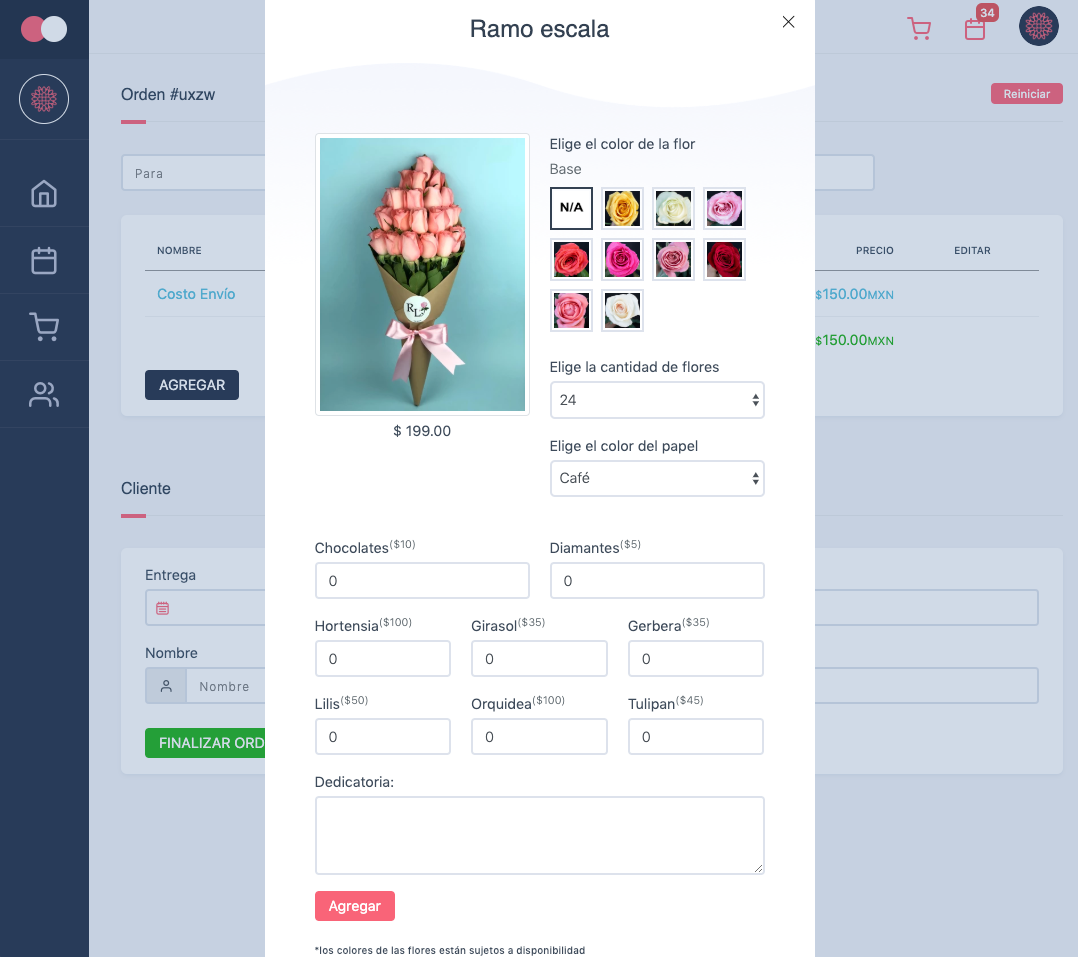
\includegraphics[width=0.6\textwidth]{app-single}
  \caption{Componente de producto.}
  \label{single-product}
\end{figure}

El componente que se utiliza para seleccionar la ubicación de destino utiliza los servicios de Google Maps. Este componente que se abre en una ventana emergente permite seleccionar un punto en un mapa, este punto esta restringido por una capa que delimita a la ciudad de Tijuana.
\vspace{0.8cm}

\begin{figure}[H]
  \centering
  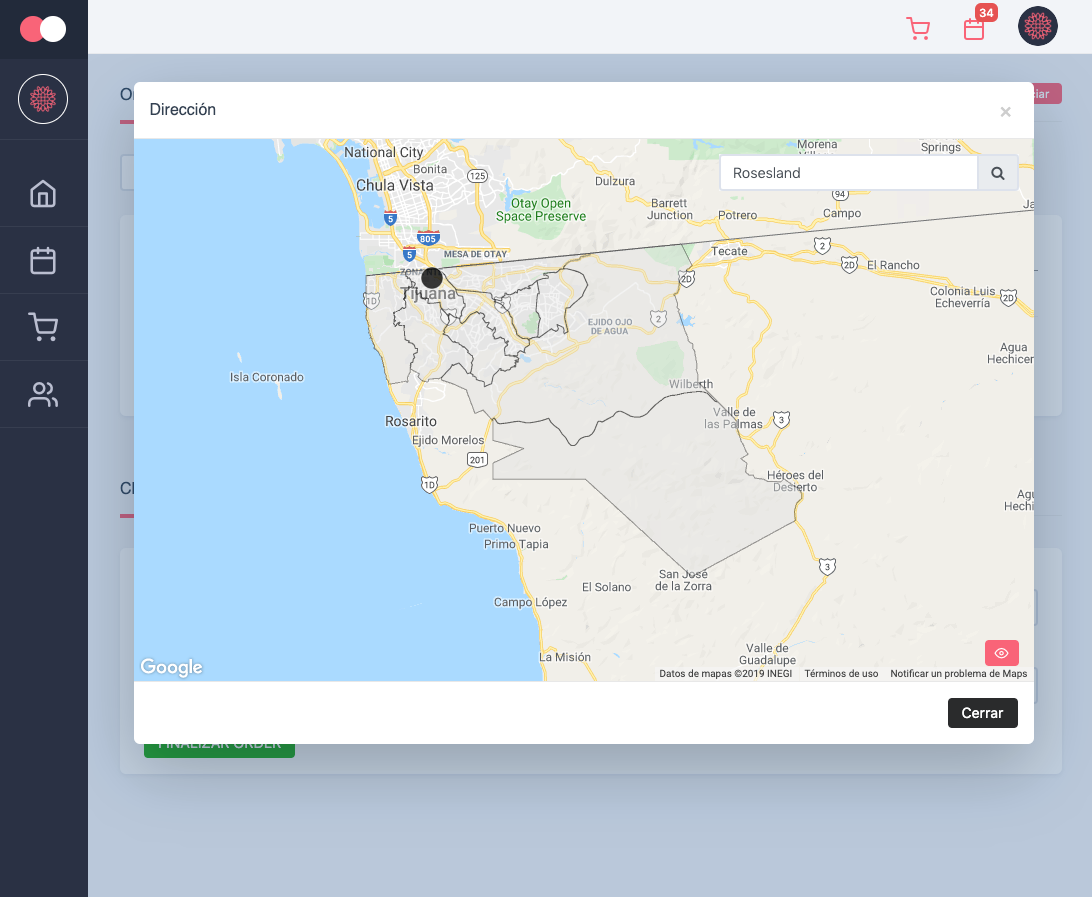
\includegraphics[width=0.8\textwidth]{app-map}
  \caption{Componente de Google Map.}
\end{figure}

Una vez seleccionada la ubicación, el sistema ejecuta una función que recibe las coordenadas y calcula la distancia entre el punto elegido y la ubicación de la florería. Para tomar en cuenta la curvatura de la tierra, esta función utiliza la fórmula del semiverseno (haversine), la cual es una ecuación importante en la navegación, proporciona distancias de entre dos puntos en una esfera desde sus longitudes y latitudes \cite{anisya}.

\[ 
  haversin\left(\frac{d}{R}\right) = haversin(\Delta\varphi) + cos(\Delta\varphi)haversin(\Delta\lambda)
\]

\textbf{Donde:}\\
\-\hspace{0.5cm} haversin es la función haversine, haversin($\Theta$) = $sen^2$ ($\Theta$/2) = (1-cos ($\Theta$))/2\\
\-\hspace{0.5cm} d es la distancia entre dos puntos\\
\-\hspace{0.5cm} R es el radio de la esfera\\
\-\hspace{0.5cm} $\Delta\varphi$ es la diferencia de latitudes\\
\-\hspace{0.5cm} $\Delta\lambda$ es la diferencia de longitudes
\vspace{0.8cm}

\lstinputlisting[style=ES6, label=login, caption=Función para calcular distancia entre dos puntos geográficos]{code/harvesine.js}

\subsubsection{Interfaz para el área de manufactura y entrega}
En esta sección se muestra el detalle de las ordenes, su principal función es desplegar en pantalla la información necesaria para elaborar y entregar los pedidos. Esta parte de la aplicación es visible para todos los usuarios, pero la información mostrada es distinta para cada empleado. Los floristas y chóferes solo pueden ver las ordenes asignadas a su usuario, los administradores y empleados de venta tienen acceso a todas las ordenes, debido a que en esta sección se encuentran los enlaces para editar las ordenes e imprimir los recibos en caso de ser solicitados.
\vspace{0.8cm}

\begin{figure}[H]
  \centering
  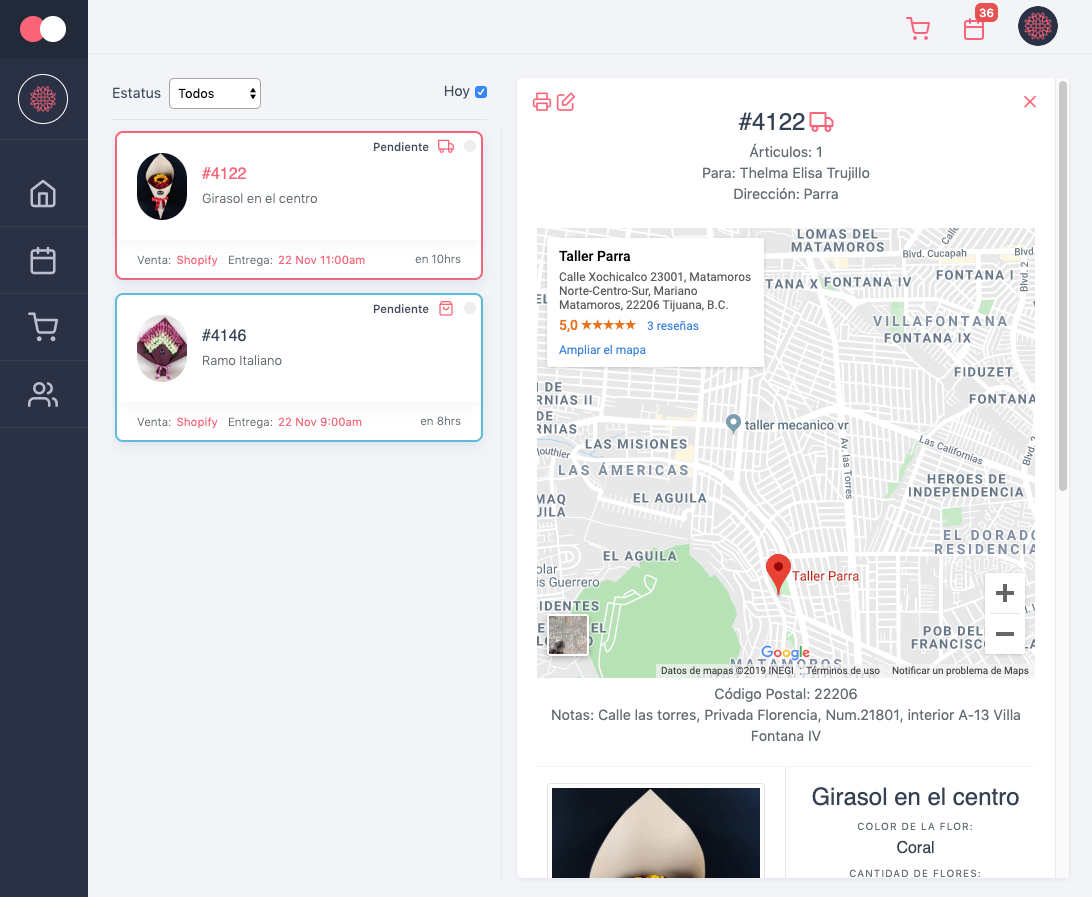
\includegraphics[width=1\textwidth]{app-orders}
  \caption{Diseño final de la sección de manufactura y entrega.}
  \label{production-ui}
\end{figure}

En la figura \ref{production-ui} se observan dos módulos principales; en el lado izquierdo se tiene una lista con las ordenes del día organizadas por hora de entrega, además de opciones para ver todas las fechas y/o filtrarlas por estatus. El lado derecho consta de un mapa con la dirección de entrega (invisible para los floristas o en caso de que la orden sea para recoger en la florería) y un tablero con las especificaciones de la orden incluidas las imágenes de los arreglos para proporcionar una ayuda visual en el área de elaboración de productos.
\vspace{0.8cm}

\subsubsection{Interfaz de administración de usuarios}
Este panel permita agregar y editar la información de los usuarios incluidos sus permisos, solo los administradores tienen acceso a este módulo; a diferencia del módulo de inicio de sesión, las actividades realizadas en estos componentes deben ser validadas por Firebase Authentication en el lado del servidor.
\vspace{0.8cm}

\begin{figure}[H]
  \centering
  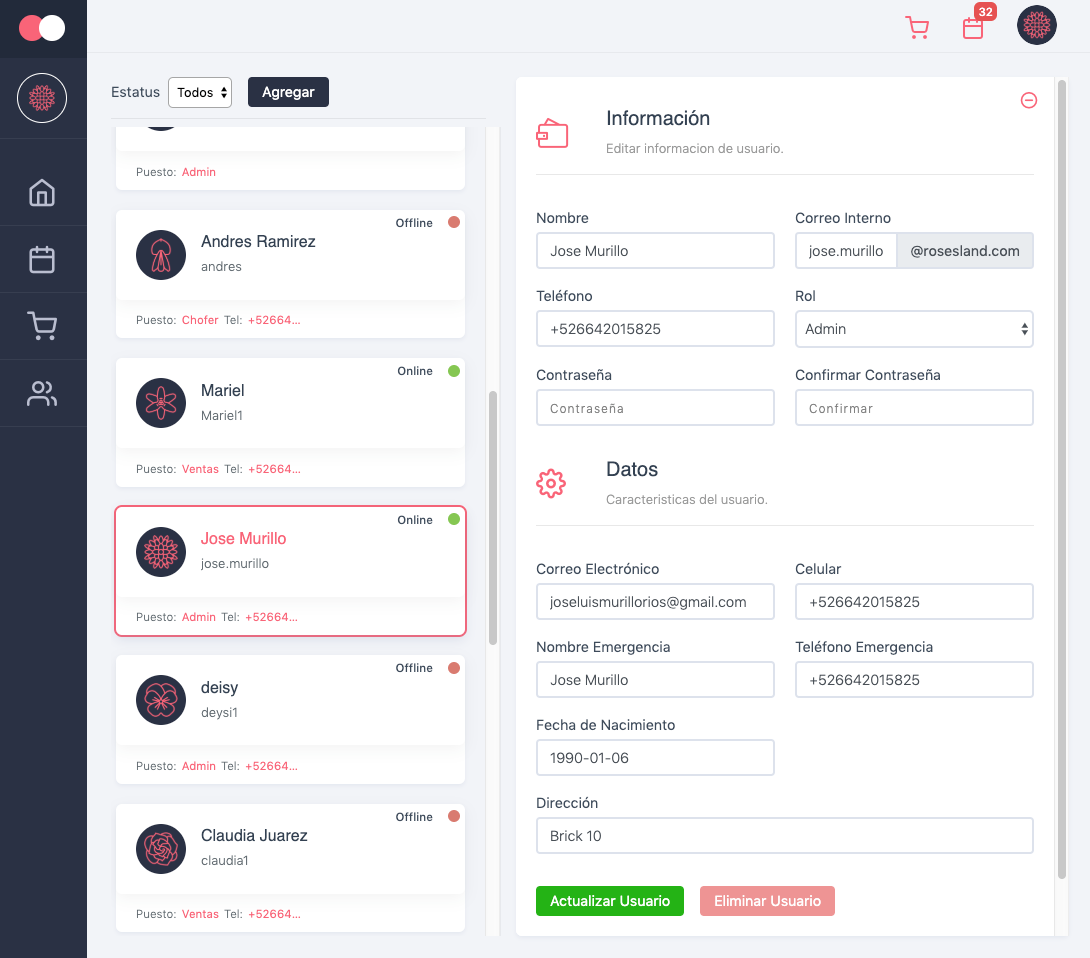
\includegraphics[width=1\textwidth]{app-admin}
  \caption{Diseño final de la sección de administración de usuarios.}
  \label{admin-ui}
\end{figure}

Por el lado izquierdo se tiene una lista con los usuarios con un indicador del estatus de su conexión en el sistema; en color rojo se muestran los empleados inactivos y en verde los empleados conectados al sistema. En el lado derecho se encuentran los campos con la información del usuario y la opción de actualizarlo o eliminarlo. En esta sección se aprecia con todo detalle los beneficios de utilizar Redux y el Diseño Atómico, distintos componentes conectados con un mismo estado (figura \ref{admin-atomic}).
\vspace{0.8cm}

\begin{figure}[H]
  \centering
  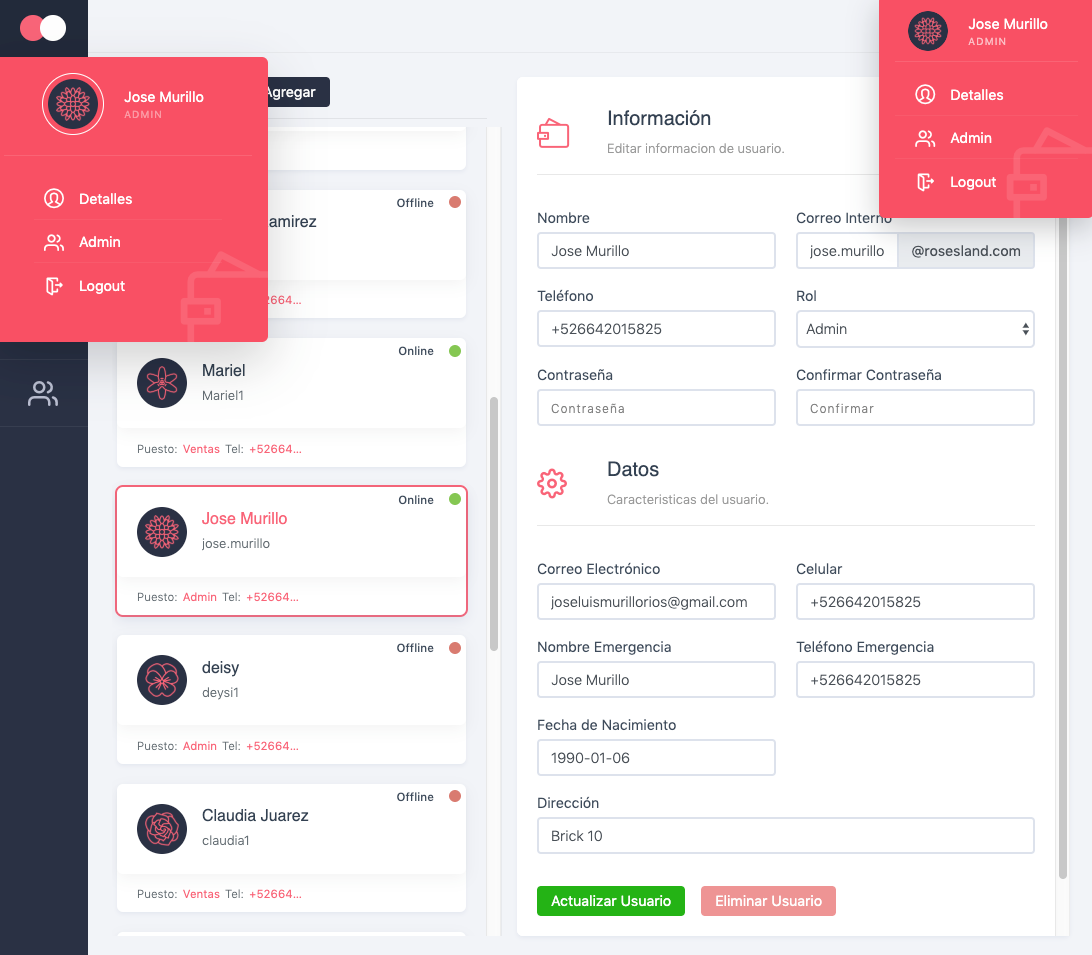
\includegraphics[width=1\textwidth]{app-atomic}
  \caption{Implementación Redux y Diseño Atómico.}
  \label{admin-atomic}
\end{figure}

\subsubsection{Evaluación de la interfaz de usuario}
El objetivo del proyecto es señalar los problemas y desafíos que surgen del uso de una pantalla táctil como dispositivo de entrada en una aplicación web. Para lograr esto, se desarrolló un prototipo, basado en pautas teóricas. El prototipo fue evaluado en sesiones informales donde los usuarios lo probaron y hablaron sobre cómo lo percibieron. Se alentó a los sujetos a sugerir soluciones alternativas y criticar las soluciones que encontraron negativas.
\vspace{0.8cm}

El prototipo inicial sufrió muy pocos cambios, siendo principalmente por motivos de funcionalidad y no estéticos. Todos los empleados que sometieron a prueba la aplicación acordaron que el diseño era fácil de entender y se podían acostumbrar a el rápidamente. El resultado de la evaluación demostró que la interfaz responsiva en una pantalla táctil genera una ayuda visual importante en todas las áreas de la empresa.